%==============================================================================
% Figure: Metric to Gravity Conceptual Map
% Purpose: Visualize logical progression from metric tensor to gravitational physics
% Chapter: Ch01 - Mathematical Preliminaries
% Type: Conceptual map / Dependency diagram
%==============================================================================

\begin{figure}[htbp]
  \centering
  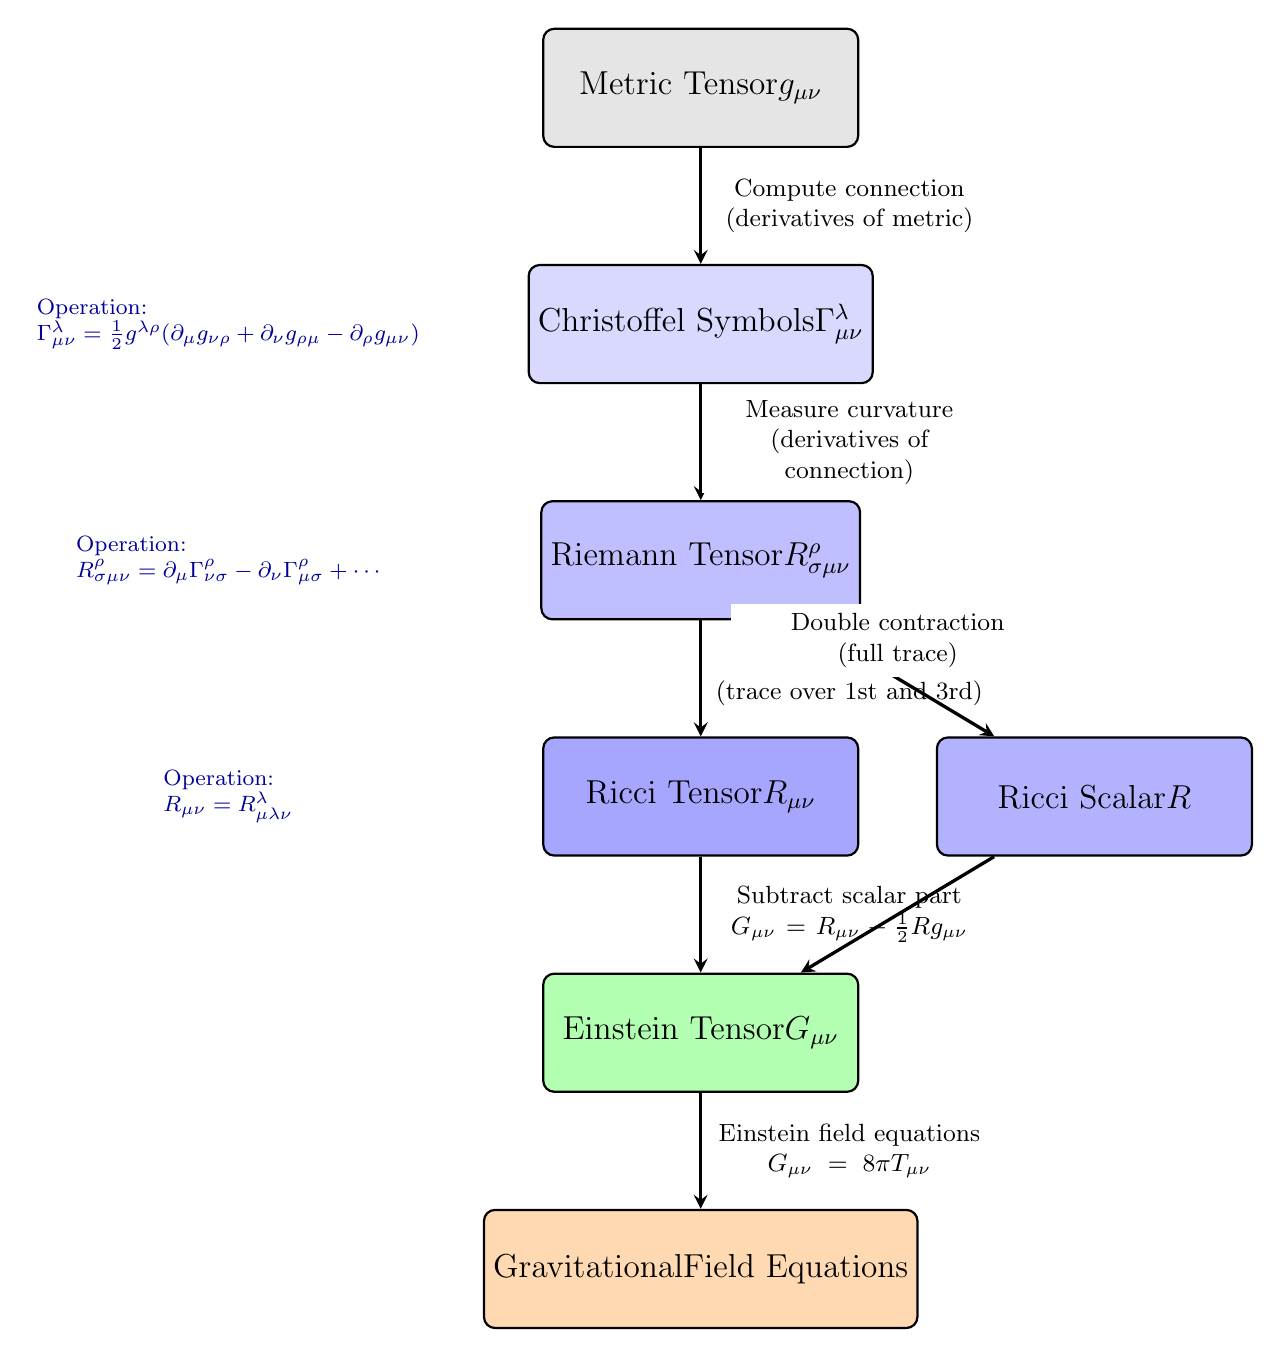
\begin{tikzpicture}[
    node distance=3cm,
    concept/.style={
      rectangle,
      rounded corners,
      minimum width=4cm,
      minimum height=1.5cm,
      text centered,
      draw=black,
      line width=0.8pt,
      font=\large
    },
    arrow/.style={
      thick,
      ->,
      >=stealth,
      line width=1.2pt
    },
    label/.style={
      font=\small,
      text width=3.5cm,
      align=center,
      fill=white
    }
  ]

    % Top row: Starting point
    \node (metric) [concept, fill=gray!20] {Metric Tensor\\$g_{\mu\nu}$};

    % Second row: Christoffel symbols
    \node (christoffel) [concept, below of=metric, fill=blue!15] {Christoffel Symbols\\$\Gamma^{\lambda}_{\mu\nu}$};

    % Third row: Riemann curvature
    \node (riemann) [concept, below of=christoffel, fill=blue!25] {Riemann Tensor\\$R^{\rho}_{\sigma\mu\nu}$};

    % Fourth row: Ricci tensor and scalar
    \node (ricci) [concept, below of=riemann, fill=blue!35] {Ricci Tensor\\$R_{\mu\nu}$};
    \node (scalar) [concept, right of=ricci, node distance=5cm, fill=blue!30] {Ricci Scalar\\$R$};

    % Fifth row: Einstein tensor
    \node (einstein) [concept, below of=ricci, fill=green!30] {Einstein Tensor\\$G_{\mu\nu}$};

    % Bottom row: Physical interpretation
    \node (gravity) [concept, below of=einstein, fill=orange!30] {Gravitational\\Field Equations};

    % Arrows with labels
    \draw [arrow] (metric) -- node[right, label] {Compute connection\\(derivatives of metric)} (christoffel);

    \draw [arrow] (christoffel) -- node[right, label] {Measure curvature\\(derivatives of connection)} (riemann);

    \draw [arrow] (riemann) -- node[right, label] {Contract indices\\(trace over 1st and 3rd)} (ricci);

    \draw [arrow] (riemann) -- node[above, label, text width=4cm] {Double contraction\\(full trace)} (scalar);

    \draw [arrow] (ricci) -- node[right, label] {Subtract scalar part\\$G_{\mu\nu} = R_{\mu\nu} - \frac{1}{2}Rg_{\mu\nu}$} (einstein);

    \draw [arrow] (scalar) -- (einstein);

    \draw [arrow] (einstein) -- node[right, label] {Einstein field equations\\$G_{\mu\nu} = 8\pi T_{\mu\nu}$} (gravity);

    % Side annotations showing mathematical operations
    \node[font=\footnotesize, text=blue!60!black, align=left, left of=christoffel, node distance=6cm]
      (op1) {Operation:\\$\Gamma^{\lambda}_{\mu\nu} = \frac{1}{2}g^{\lambda\rho}(\partial_{\mu}g_{\nu\rho} + \partial_{\nu}g_{\rho\mu} - \partial_{\rho}g_{\mu\nu})$};

    \node[font=\footnotesize, text=blue!60!black, align=left, left of=riemann, node distance=6cm]
      (op2) {Operation:\\$R^{\rho}_{\sigma\mu\nu} = \partial_{\mu}\Gamma^{\rho}_{\nu\sigma} - \partial_{\nu}\Gamma^{\rho}_{\mu\sigma} + \cdots$};

    \node[font=\footnotesize, text=blue!60!black, align=left, left of=ricci, node distance=6cm]
      (op3) {Operation:\\$R_{\mu\nu} = R^{\lambda}_{\mu\lambda\nu}$};

  \end{tikzpicture}

  \caption{Conceptual map showing the logical progression from metric tensor to gravitational physics in General Relativity. Each step involves specific differential operations on the previous structure, building from the fundamental metric $g_{\mu\nu}$ (which encodes spacetime geometry) through increasingly abstract curvature tensors, culminating in Einstein's field equations. This hierarchy demonstrates how geometry becomes physics.}
  \label{fig:metric-to-gravity}
\end{figure}
